\newif\ifnotes

% Uncomment either one to render the document with or without notes
%\notestrue
\notesfalse

% Adjust beamer template
\documentclass[aspectratio=169,xcolor=dvipsnames]{beamer}

\usetheme{Simple}

\setbeamertemplate{footline}[frame number]{} % Use frame numbers instead of page numbers
\ifnotes
    \setbeamertemplate{note page}[plain]
    \setbeameroption{show notes on second screen=bottom}
\fi

\usepackage{hyperref}
\usepackage{graphicx}
\usepackage{booktabs}

\usepackage[outputdir=build]{minted}

% Overwrite minted style
\setminted[Rust]{
    breaklines=true,
    escapeinside=''
}

\usemintedstyle{manni}

% Macro color for overwriting if the macro is not recognized
\definecolor{macro}{rgb}{0.80, 0.00, 1.00}

% Commands
\newcommand{\rust}[1]{\mintinline{rust}{#1}}
\newcommand{\nohighlight}[1]{\mintinline{TeX}{#1}}
\newcommand{\enote}[1]{
    \note{
        \textbf{Notes:}
        \begin{enumerate}
            #1
        \end{enumerate}
    }
}
\newcommand{\so}{$\rightarrow$ }
\newcommand{\br}{\vspace{\baselineskip}}

% !TeX root = ../main.tex
\title[Rust for Network Servers]{Rust for Network Servers}
\subtitle{Synchronous and asynchronous network communication}

\author[Simon Pannek] {Simon Pannek}
\institute[TUM]{
    Technical University of Munich \\
    Munich, Germany
    \vskip 3pt
}
\date{\today}


\begin{document}

% Title
\begin{frame}
    \titlepage
\end{frame}

% Slides
% !TeX root = ../main.tex
\begin{frame}{Introduction}
    \center{Back in the 1960s the protocols for one of the first computer networks were developed.}
    \begin{figure}
        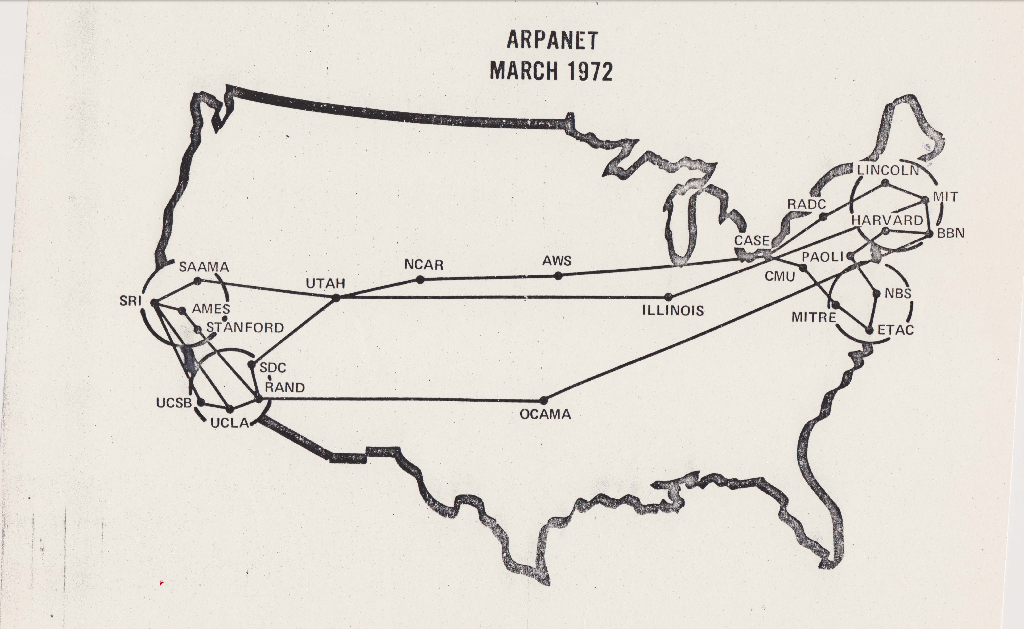
\includegraphics[width=0.5\linewidth]{images/arpanet_1972.png}
        \caption{Ferris the Crab \cite{arpanet}}
    \end{figure}

    \enote{
        \item Many modern devices used today are using the internet to communicate with each other
        \item A foundation for this can be found when looking at the ARPANET
        \item ARPANET: A packet-switching network deployed in the US
        \begin{enumerate}
            \item One of the first networks to implement the TCP/IP protocol suite
            \item Evolved into the Internet as we know it today
        \end{enumerate}
    }
\end{frame}

% !TeX root = ../main.tex
\begin{frame}{Introduction}
    \textbf{What happened until now?}
    \begin{enumerate}
        \item<1-> Additional security (encryption)
        \item<2-> Introduction of new protocols
        \item<3> A lot was standardized (IEEE standards, W3C, ...)
    \end{enumerate}
\end{frame}

% !TeX root = ../main.tex
\begin{frame}{Introduction}
    \Huge
    \centerline{What programming language to choose?}

    \enote{
        \item Standardization \so common used programming language usually support frequently deployed networking
        protocols
        \item Depends on the use case: Certain trade offs comparing different languages
        \item We are going to take a look at Rust and what it has to offer when it comes to running it as a backend of
        a network application
    }
\end{frame}

% !TeX root = ../main.tex
\begin{frame}[fragile]{Introduction}
    \begin{enumerate}
        \item[]<2> \Huge
        \centerline{Buffer Overflow Attacks}

        \item[]<1-> \Large
        \begin{minted}{C}
            void unsecure_function(void) {
                char buf[512];
                read_from_network(buf);

                ...
            }
        \end{minted}
    \end{enumerate}

    \enote{
        \item Let us take a step back: Currently, many networking libraries are written in C or C++
        \item What is the problem with this piece of code?
        \item Buffer overflow attacks (Small explanation what can happen)
        \item No guaranteed memory safety in C and C++
        \item Mistakes of a programmer are not checked by the compiler and fall back to some default action (UB \so
        corruption of memory)
        \item Problematic for network applications (many concurrent reads and writes to buffers)
    }
\end{frame}

% !TeX root = ../main.tex
\begin{frame}[fragile]{Introduction}
    \begin{enumerate}
        \item[]<2> \Huge
        \centerline{Interpreted languages}

        \item[]<1-> \Large
        \begin{minted}{Python}
            def more_secure_function(socket):
                buf = socket.recv(512)
    
                ...
        \end{minted}
    \end{enumerate}

    \enote{
        \item Simplified example \so Depends on the actual use case and implementation whether something can be
        considered secure
        \item Interpreted languages like Python as a solution (background checks for undefined behavior for almost
        everything)
        \item Scripting languages allow fast prototyping
        \item Trade off of interpreted languages: Slower performanced compared to executing compiled binary files
        (Instructions first have to get translated by the interpreter)
        \item They do not run natively on the computer \so you first have to install the interpreter
    }
\end{frame}

% !TeX root = ../main.tex
\begin{frame}{Introduction}
    \Huge
    \centerline{Rust as a solution?}

    \br

    \begin{figure}
        
\includegraphics[width=0.3\linewidth]{images/ferris.png}
        \caption{Ferris the Crab \cite{ferris}}
    \end{figure}

    \enote{
        \item Rust can be considered "the best of both worlds":
        \begin{enumerate}
            \item Compiled language with a compiler guaranteeing memory- and thread-safety
            \item Fast speed of compiled languages and prevents most of the vulnerabilities mentioned before through
                  its compiler checks
            \item Network operations are prune to failure \so unsafe calls can be wrapped into enums of the type
                  \rust{std::result::Result}
            \item Package manager Cargo
        \end{enumerate}
        \item Let us first take a look how to implement basic TCP and UDP communication in Rust
    }
\end{frame}


% !TeX root = ../main.tex
\begin{frame}{Networking in Rust}
    \Huge
    \centerline{Ownership, borrowing, and lifetimes}

    \pause

    \br

    \Large
    \centerline{\so No dangling references, illegal memory access, and memory leaks}

    \pause

    \br

    \small
    \centerline{(Except if you are explicitly working with \rust{unsafe} code)}

    \enote{
        \item Ownership, borrowing and lifetimes play an important role in networking code
        \item Ownership:
        \begin{enumerate}
            \item A part of the code can own a piece of memory
            \item Function is called with an owned value \so the piece of memory gets moved into that function
        \end{enumerate}
        \item Borrowing:
        \begin{enumerate}
            \item No complete access is needed \so a reference can be borrowed
            \item There are also mutable reference: Only one is allowed at the same time
            \item Useful whne working with network applications (prevents the occurence of data races if a thread tires
                  to read or write to a buffer while another thread is already writing to it)
            \item We are not going to take a look at \rust{std::sync::Arc}
        \end{enumerate}
        \item Lifetimes:
        \begin{enumerate}
            \item Lifetime determined by the code block it was created \so variable gets out of scope \so the
                  corresponding piece of memory is freed
            \item If a value gets moved into another function, its lifetime changes with it
        \end{enumerate}
    }
\end{frame}

% !TeX root = ../main.tex
\begin{frame}{Networking in Rust}
    \textbf{The Transmission Control Protocol (TCP)}

    \begin{itemize}
        \item<2-> Active connection between two systems
        \item<3-> Can be used to send a continous stream of octets to another host
        \item<4-> A sequence number is assigned to each octet in order to confirm it was received
        \item<5> If no acknowledgment (ACK) was received, the data is sent again
    \end{itemize}

    \enote{
        \item TCP is used for reliable inter-process communication between two systems connected through a network
        \item The sequence number can also be used to eliminate duplicates
        \item \rust{std::net} module includes networking functions for TCP
    }
\end{frame}

% !TeX root = ../main.tex
\begin{frame}[fragile]{Networking in Rust}
    \begin{block}{TCP client handeling}
        \begin{overprint}
            \onslide<1>
            \begin{minted}{Rust}
            let mut reader = BufReader::new(&stream);
            
            loop {
                let mut buf = String::new();
            
                match reader.read_line(&mut buf) {
                    '\Large{...}'
                }
            }
            \end{minted}

            \onslide<2>
            \begin{minted}{Rust}
            match reader.read_line(&mut buf) {
                Ok(0) => break,
                Ok(_) => print!("{}", buf),
                Err(e) => {
                    eprintln!("{}", e);
                    stream.shutdown(Both)?;
                    break;
                }
            }
            \end{minted}
        \end{overprint}
    \end{block}
\end{frame}

% !TeX root = ../main.tex
\begin{frame}[fragile]{Networking in Rust}

    \begin{block}{TCP listener}
        \begin{minted}{Rust}
            let listener = TcpListener::bind(ADDRESS)
                .expect("Bind to address");
            
            for stream in listener.incoming() {
                if let Ok(stream) = stream {
                    handle_client(stream)
                        .expect("Handle client");
                }
            }
        \end{minted}
    \end{block}
\end{frame}

% !TeX root = ../main.tex
\begin{frame}[fragile]{Networking in Rust}

    \begin{block}{TCP client}
        \begin{overprint}
            \onslide<1>
            \begin{minted}{Rust}
            let mut stream = TcpStream::connect(ADDRESS)?;

            loop {
                let mut buf = String::new();
            
                match stdin().read_line(&mut buf) {
                    '\Large{...}'
                }
            }
            \end{minted}

            \onslide<2>
            \begin{minted}{Rust}
                match stdin().read_line(&mut buf) {
                    Ok(_) => {
                        '\Large{...}'
                    }
                    Err(e) => {
                        eprintln!("{}", e);
                        stream.shutdown(Both)?;
                        break;
                    }
                }
            \end{minted}

            \onslide<3>
            \begin{minted}{Rust}
                Ok(_) => {
                    let bytes = buf.as_bytes();
        
                    stream
                        .write_all(bytes)
                        .expect("Writing");
                }
            \end{minted}
        \end{overprint}
    \end{block}
\end{frame}


% !TeX root = ../main.tex
\begin{frame}{Networking in Rust}
    \textbf{The User Datagram Protocol (UDP)}
    \begin{itemize}
        \item<2-> Commonly used if you do not need reliable delivery of streams
        \item<3-> Tries to send messages to other programs with a minimal amount of protocol mechanism
        \item<4-> No protection against package duplication
        \item<5> No checks whether the data sent has arrived and if it did in what order
    \end{itemize}

    \enote{
        \item UDP is less reliable than the Transmission Control Protocol
        \item No need to listen for new hosts or actively establish a connection
        \item Typical example: Media streaming (package loss is acceptable)
    }
\end{frame}

% !TeX root = ../main.tex
\begin{frame}[fragile]{Networking in Rust}

    \begin{block}{UDP receiver}
        \begin{overprint}
            \onslide<1>
            \begin{minted}{Rust}
            let socket = UdpSocket::bind(ADDRESS)?;

            loop {
                let mut buf = [0u8; 1500];
            
                match socket.recv_from(&mut buf) {
                    '\Large{...}'
                }
            }
            \end{minted}

            \onslide<2>
            \begin{minted}{Rust}
            match socket.recv_from(&mut buf) {
                Ok(_) => {
                    let msg = from_utf8(&buf)
                        .expect("Convert data");
        
                    print!("{}", msg);
                }
                Err(e) => {
                    eprintln!("{}", e);
                    break;
                }
            }
            \end{minted}
        \end{overprint}
    \end{block}

    \enote{
        \item Why is the buffer size 1500? (Maximum Transmission Unit)
        \item Why is a buffer needed at all? (\rust{std::net::UdpSocket} does not implement the trait
        \rust{std::io::Read})
    }
\end{frame}

% !TeX root = ../main.tex
\begin{frame}[fragile]{Networking in Rust}
    \begin{block}{UDP sender}
        \begin{overprint}
            \onslide<1>
            \begin{minted}{Rust}
            let socket = UdpSocket::bind("0.0.0.0:0")?;

            loop {
                let mut buf = String::new();
            
                match stdin().read_line(&mut buf) {
                    '\Large{...}'
                }
            }
            \end{minted}

            \onslide<2>
            \begin{minted}{Rust}
            match stdin().read_line(&mut buf) {
                Ok(_) => {
                    let bytes = buf.as_bytes();
        
                    socket
                        .send_to(bytes, ADDRESS)
                        .expect("Sending");
                }
                Err(e) => {
                    eprintln!("{}", e);
                    break;
                }
            }
            \end{minted}
        \end{overprint}
    \end{block}
\end{frame}


% !TeX root = ../main.tex
%\begin{frame}{Overview}
% Throughout your presentation, if you choose to use \section{} and \subsection{} commands, these will automatically be printed on this slide as an overview of your presentation
%    \tableofcontents
%\end{frame}

%------------------------------------------------
\section{First Section}
%------------------------------------------------

\begin{frame}{Bullet Points}
    \begin{itemize}
        \item Lorem ipsum dolor sit amet, consectetur adipiscing elit
        \item Aliquam blandit faucibus nisi, sit amet dapibus enim tempus eu
        \item Nulla commodo, erat quis gravida posuere, elit lacus lobortis est, quis porttitor odio mauris at libero
        \item Nam cursus est eget velit posuere pellentesque
        \item Vestibulum faucibus velit a augue condimentum quis convallis nulla gravida
    \end{itemize}
\end{frame}

%------------------------------------------------

\begin{frame}{Enumerating Bullet Points}
    \begin{enumerate}
        \item<1-> First bullet
        \item<3> This is the last bullet
        \item<2-> This bullet appears second
    \end{enumerate}
\end{frame}

%------------------------------------------------

\begin{frame}{Blocks of Highlighted Text}
    In this slide, some important text will be \alert{highlighted} because it's important. Please, don't abuse it.

    \begin{block}{Block}
        Sample text
    \end{block}

    \begin{alertblock}{Alertblock}
        Sample text in red box
    \end{alertblock}

    \begin{examples}
        Sample text in green box. The title of the block is ``Examples".
    \end{examples}
\end{frame}

%------------------------------------------------

\begin{frame}{Multiple Columns}
    \begin{columns}[c] % The "c" option specifies centered vertical alignment while the "t" option is used for top vertical alignment

        \column{.45\textwidth} % Left column and width
        \textbf{Heading}
        \begin{enumerate}
            \item Statement
            \item Explanation
            \item Example
        \end{enumerate}

        \column{.5\textwidth} % Right column and width
        Lorem ipsum dolor sit amet, consectetur adipiscing elit. Integer lectus nisl, ultricies in feugiat rutrum, porttitor sit amet augue. Aliquam ut tortor mauris. Sed volutpat ante purus, quis accumsan dolor.

    \end{columns}
\end{frame}

%------------------------------------------------
\section{Second Section}
%------------------------------------------------

\begin{frame}{Table}
    \begin{table}
        \begin{tabular}{l l l}
            \toprule
            \textbf{Treatments} & \textbf{Response 1} & \textbf{Response 2} \\
            \midrule
            Treatment 1         & 0.0003262           & 0.562               \\
            Treatment 2         & 0.0015681           & 0.910               \\
            Treatment 3         & 0.0009271           & 0.296               \\
            \bottomrule
        \end{tabular}
        \caption{Table caption}
    \end{table}
\end{frame}

%------------------------------------------------

\begin{frame}{Theorem}
    \begin{theorem}[Mass--energy equivalence]
        $E = mc^2$
    \end{theorem}
\end{frame}

%------------------------------------------------

\begin{frame}{Figure}
    Uncomment the code on this slide to include your own image from the same directory as the template .TeX file.
    %\begin{figure}
    %\includegraphics[width=0.8\linewidth]{test}
    %\end{figure}
\end{frame}

%------------------------------------------------

\begin{frame}[fragile] % Need to use the fragile option when verbatim is used in the slide
    \frametitle{Citation}
    An example of the \verb|\cite| command to cite within the presentation:\\~

    This statement requires citation \cite{p1}.
\end{frame}

%------------------------------------------------

\begin{frame}
    \Huge{\centerline{The End}}
\end{frame}


% References
\begin{frame}{References}
    \begin{columns}[c]

        % Left column
        \column{.5\textwidth}

        \footnotesize {
            \begin{thebibliography}{9}

                \bibitem[1]{arpanet} UCLA and BBN (1972)
                \newblock The map of ARPANET in March 1972.
                \newblock \url{https://commons.wikimedia.org/wiki/File:Arpanet_1972_Map.png}

            \end{thebibliography}
        }

        % Right column
        \column{.5\textwidth}

        \footnotesize {
            \begin{thebibliography}{9}

                \bibitem[2]{ferris} Rustacean.net
                \newblock Ferris the Crab.
                \newblock \url{https://rustacean.net/assets/rustacean-flat-happy.png}

            \end{thebibliography}
        }

    \end{columns}
\end{frame}


\end{document}
